% ============================================================
% Chapter 1 --- Prerequisites and a first look at R^n
% Originally: content/week-01.tex (no single tutor; assembled from several
%             tutors' recap slides, since Corsin's notes start a week later)
% ============================================================
\chapter{Prerequisites and a First Look at \texorpdfstring{$\mathbb{R}^n$}{Rn}}
\label{ch:prerequisites}

% Transition: Claude Opus 5 (Medium)
This chapter collects the \emph{Analysis I} material the course takes for granted, together with
the $\mathbb{R}^n$ warm-up that precedes any of its theory. It has no single tutor behind it:
Corsin's own class notes open with the second week of teaching, and no tutor's notes cover the
opening week on its own terms, since that week consists mostly of a recap and an exercise in
reading and drawing subsets of $\mathbb{R}^n$. The material below is therefore assembled from the
recap slides several tutors independently found worth revisiting. It also proves Young's
inequality (\cref{prop:youngs_inequality}), a fact used repeatedly once norms and Hölder-type
estimates appear.

% Originally: content/week-01.tex, \section{From Analysis I to several variables}
% Source: Maarten Cnoops/Woche 1.pdf, p. 1
\section{From Analysis I to several variables}
\label{sec:analysis1_recap}

Several of the definitions you will meet in the coming chapters are exactly the definitions you
already know from \emph{Analysis I}, only stripped of their reliance on the real line. A
\newterm{sequence} (\germanterm{Folge}) $(x_k)_{k \in \mathbb{N}}$ in a set $X$ converging to
$x \in X$, a function being continuous at a point, a set being open or closed --- all of these
notions carry over to $\mathbb{R}^n$ and, as \cref{sec:structured_spaces} will show, to much more
general spaces than $\mathbb{R}^n$. What does \emph{not} carry over automatically is anything
that relied on the \emph{order} of $\mathbb{R}$: there is no \qt{$\leq$} on $\mathbb{R}^n$ for
$n \geq 2$, so statements like the intermediate value theorem or \qt{every bounded sequence has a
convergent subsequence} need new proofs, or new hypotheses, once we leave $\mathbb{R}$.

\begin{remark}
That last fact --- bounded does \emph{not} imply convergent, but bounded sequences in
$\mathbb{R}^n$ do always have a convergent \emph{subsequence} --- is exactly the statement of the
Bolzano--Weierstrass theorem, revisited via \cref{ex:1.1} below. It
reappears as the Heine--Borel theorem once compactness is introduced in \cref{sec:compactness}.
\end{remark}

% Supplement: Linus Lüchinger/Slides/Slides-02-23.pdf
\begin{ainote}
Linus Lüchinger's first exercise-session slides collect the most common mistakes on the first
problem sheet, whose problems are distributed through this chapter. Two are worth flagging before
attempting \cref{ex:1.1}: on part 2, most students first guessed $f(x) = \log|x| + c$ for a single
constant $c$ --- wrong, since the two constants on $(-\infty,0)$ and $(0,\infty)$ may genuinely
differ (see \cref{sec:prerequisites_solutions}). On part 4, most students assumed a function with
everywhere-positive second derivative cannot have a global maximum; it can, at the boundary of the
domain.
\end{ainote}

% Source: exercises/Ex1_Analysis2_eng.pdf, p. 1
\begin{exercise}[1.1 --- Recap Questions]
\label{ex:1.1}
\begin{enumerate}[label=\textbf{\arabic*.}]
  \item Let $\{x_k\}_{k \in \mathbb{N}} \subset [1,2] \subset \mathbb{R}$ be a sequence. Is it
    necessarily convergent?
  \item Describe all differentiable functions $f : \mathbb{R} \setminus \{0\} \to \mathbb{R}$ such
    that $f'(x) = 1/x$ for all $x \neq 0$.
  \item Let $f : \mathbb{R} \to \mathbb{R}$ be continuous and bounded. Is it true that
    \[
      \int_0^{\pi/2} f(\cos(x))\,dx = \int_0^1 \frac{f(t)}{\sqrt{1-t^2}}\,dt \, ?
    \]
  \item Let $f : [0,\infty) \to \mathbb{R}$ have $f''(x) > 0$ for all $x \geq 0$. Can $f$ have a
    global maximum point?
  \item Let $\phi : \mathbb{R}^2 \to \mathbb{R}^2$ be a linear map and let
    $Q := [0,1] \times [0,1]$ be the unit square. How does $\phi(Q)$ look like? What are the
    possibilities?
  \item Consider the vector space $V$ of polynomials of degree less than $4$, and the function
    $D : V \to V$ which associates to a polynomial $p$ its derivative $p'$. Is $D$ a linear map?
    If so, what is the dimension of its null space?
\end{enumerate}
\end{exercise}

% Originally: content/week-01.tex, \section{Young's inequality}
% Authored for these notes around the statement of problem 1.4; no tutor's notes cover it.
\section{Young's inequality}
\label{sec:youngs_inequality}

The following inequality is not part of the lecture's main line of development, but it is the
cleanest route to comparing different norms on $\mathbb{R}^n$ (see \cref{sec:cauchy_schwarz}) and
to the Hölder-type estimates that appear whenever two $L^p$-type quantities are played off against
each other. It is worth proving once and citing from then on.

\begin{proposition}[Young's inequality]
\label{prop:youngs_inequality}
% Source: exercises/Ex1_Analysis2_eng.pdf, Problem 1.4
Let $a, b > 0$ and let $p, q > 1$ satisfy $\tfrac{1}{p} + \tfrac{1}{q} = 1$. Then
\[
  ab \leq \frac{a^p}{p} + \frac{b^q}{q}.
\]
\end{proposition}

\begin{remark}
The case $p = q = 2$ recovers the familiar inequality $ab \leq \tfrac{a^2}{2} + \tfrac{b^2}{2}$,
which is just a rewriting of $(a-b)^2 \geq 0$.
\end{remark}

\begin{proof}
Fix conjugate exponents $p, q > 1$, and define $g : (0,\infty) \to \mathbb{R}$ by
$g(t) := \tfrac{t}{p} + \tfrac{1}{q} - t^{1/p}$. We first show that $g \geq 0$, with equality only
at $t = 1$. Differentiating,
\[
  g'(t) = \frac{1}{p}\left(1 - t^{-(p-1)/p}\right).
\]
Since $p > 1$, the exponent $-(p-1)/p$ is negative, so $t^{-(p-1)/p} > 1$ for $t \in (0,1)$ and
$t^{-(p-1)/p} < 1$ for $t > 1$. Hence $g' < 0$ on $(0,1)$ and $g' > 0$ on $(1,\infty)$, so $g$
attains a global minimum at $t = 1$. As $g(1) = \tfrac{1}{p} + \tfrac{1}{q} - 1 = 0$, we obtain
\begin{equation}
\label{eq:young_scalar_key}
  t^{1/p} \leq \frac{t}{p} + \frac{1}{q} \qquad \text{for all } t > 0.
\end{equation}
Now fix $a, b > 0$ and apply \eqref{eq:young_scalar_key} with $t := a^p / b^q$. Multiplying both
sides by $b^q > 0$ gives
\[
  \left(\frac{a^p}{b^q}\right)^{1/p} b^q \ \leq\ \frac{a^p}{p} + \frac{b^q}{q}.
\]
It remains to identify the left-hand side, and this is where the conjugacy of $p$ and $q$ enters.
Using $1 - \tfrac{1}{p} = \tfrac{1}{q}$,
\[
  \left(\frac{a^p}{b^q}\right)^{1/p} b^q
    \ =\ a\,b^{-q/p}\,b^{q}
    \ =\ a\,b^{\,q\left(1 - \frac{1}{p}\right)}
    \ =\ a\,b^{\,q \cdot \frac{1}{q}}
    \ =\ ab,
\]
which is exactly the asserted inequality.
\end{proof}

% Generator: Claude Opus 5 (High)
\begin{remark}[From Young to Hölder]
\label{rem:young_to_hoelder}
The exercise sheet also asks for the vector version
\begin{equation}
\label{eq:young_vector}
  \langle a,b\rangle \leq \frac{\|a\|_p^p}{p} + \frac{\|b\|_q^q}{q}, \qquad a,b \in \mathbb{R}^n,
\end{equation}
where $\|x\|_p := \left(\sum_i |x_i|^p\right)^{1/p}$. This is \emph{not} yet Hölder's inequality:
it is the scalar case applied coordinatewise and summed (see the solution of \cref{ex:1.4}
below), and the right-hand side is a sum of $p$-th and $q$-th powers rather than the product
$\|a\|_p\|b\|_q$. The step from one to the other is a normalisation, and it is worth seeing
once, because the same trick recurs whenever an inequality is homogeneous.

Assume $a,b \neq 0$ and apply \eqref{eq:young_vector} to the rescaled vectors
$a/\|a\|_p$ and $b/\|b\|_q$, each of which has $p$- resp.\ $q$-norm equal to $1$:
\[
  \frac{\langle a,b\rangle}{\|a\|_p\,\|b\|_q} \ \leq\ \frac{1}{p} + \frac{1}{q} \ =\ 1,
\]
which is exactly \newterm{Hölder's inequality} \germanfor{Höldersche Ungleichung}
$\langle a,b\rangle \leq \|a\|_p\|b\|_q$. The conjugacy condition
$\tfrac1p+\tfrac1q=1$, which so far looked like an arbitrary bookkeeping device, is what makes
the two constants add up to exactly $1$ here.

This is also a first hint of why $p$-norms other than $p=2$ are worth naming:
\Cref{sec:cauchy_schwarz} only treats $p = q = 2$, where Hölder's inequality is
Cauchy--Schwarz, but the same machinery bounds $\langle a, b\rangle$ for every conjugate pair
$(p,q)$.
\end{remark}

% Source: exercises/Ex1_Analysis2_eng.pdf, p. 2
\begin{exercise}[1.4 --- Young's inequality]
\label{ex:1.4}
Let $a,b > 0$, and let $p,q>1$ with $\tfrac{1}{p}+\tfrac{1}{q}=1$. Prove that
$ab \leq \tfrac{a^p}{p} + \tfrac{b^q}{q}$.
\begin{enumerate}[label=\textbf{\arabic*.}]
  \item Prove that for all $t>0$, $t^{1/p} \leq \tfrac{t}{p} + \tfrac{1}{q}$.
  \item Multiply the inequality by $b^q$ and choose an appropriate value of $t$ to conclude.
\end{enumerate}
\textbf{A bonus:} show that $\langle a,b\rangle \leq \tfrac{\|a\|_p^p}{p} + \tfrac{\|b\|_q^q}{q}$
for all $a,b \in \mathbb{R}^n$.
\end{exercise}

% Originally: content/week-01.tex, \section{Visualizing sets in R^2 and R^3}
% Authored for these notes; no single source. The remark at the end of the section draws on
% several tutors' opening-week slides (the live Desmos 3D / GeoGebra demonstrations).
\section{Visualizing sets in \texorpdfstring{$\mathbb{R}^2$}{R2} and \texorpdfstring{$\mathbb{R}^3$}{R3}}
\label{sec:visualizing_sets}

Much of the geometric intuition for this course --- open sets, level sets, submanifolds --- rests
on a skill that has nothing to do with any theorem: reading a set-builder description and
producing an accurate picture, or going the other way. Two techniques are worth naming
explicitly, both used repeatedly in the solutions below.

\begin{itemize}
  \item \textbf{Slicing.} To sketch a set $S \subseteq \mathbb{R}^3$ defined by an equation
    involving $z$, fix $z = t$ and sketch the resulting planar slice $S \cap \{z = t\}$ as $t$
    varies. Stacking the slices gives the full picture.
  \item \textbf{Level sets.} If a set is defined by $f(x,y) = t$ for a fixed $t$, first work out
    the level sets $\{f = t\}$ of $f$ for varying $t$; many natural functions (e.g.
    $f(x,y) = \max\{|x|,|y|\}$, whose level sets are squares, or $f(x,y) = \sqrt{x^2+y^2}$, whose
    level sets are circles) have level sets that are easy to name, which turns a 3D sketch into a
    stack of named 2D shapes.
\end{itemize}

Both techniques are applied to \cref{ex:1.2,ex:1.3} below, and worked out in
\cref{sec:prerequisites_solutions}.

\begin{remark}
Several tutors' slides (e.g.\ those using Desmos 3D or GeoGebra to plot these sets live) note that
students commonly guess the wrong growth rate for sets like
$\{(x,y,z) : z = \sqrt{1+x^2+y^2}\}$, sketching a cone instead of a hyperboloid-like bowl that
steepens towards slope $1$; the slicing technique above makes the mistake visible immediately, since the slice
at height $t$ only exists for $t \geq 1$ and has radius $\sqrt{t^2-1}$, not $t$.
\end{remark}

% Source: exercises/Ex1_Analysis2_eng.pdf, p. 1
\begin{exercise}[1.2 --- From equations to drawings]
\label{ex:1.2}
Sketch the following subsets of $\mathbb{R}^2$, $\mathbb{R}^3$.
\begin{enumerate}[label=\textbf{\arabic*.}]
  \item $A := \{(x,y) : x^2+y^2 < 1,\ y \geq x^2\}$
  \item $B := \{(x,y) : y^2 = x^3 - x\}$
  \item $C := \{(x,y) : \tfrac{\pi}{6} < \arctan(y/x) < \tfrac{\pi}{3},\ 0 < x < y\}$
  \item $D := \{(x,y,z) : \sqrt{x^2+y^2} = 1-z,\ 0 < z < 1\}$
  \item $E := \{(x,y,z) : z = \sqrt{1+x^2+y^2}\}$
  \item $F := \{(x,y,z) : z = \max\{|x|,|y|\}\}$
\end{enumerate}
\end{exercise}

% Source: exercises/Ex1_Analysis2_eng.pdf, p. 1
\begin{exercise}[1.3 --- From drawings to equations]
\label{ex:1.3}
Express in terms of functions and equations the following sets.
\begin{enumerate}[label=\textbf{\arabic*.}]
  \item The coordinates of a point in the plane that goes endlessly back and forth from the
    origin to the point $(-1,1)$.
  \item A planar domain with two holes in it.
  \item A bi-dimensional disk sitting inside the plane $\{x+y+z=0\}$ in $\mathbb{R}^3$.
  \item A Pac-Man shaped domain in the plane.
  \item A pyramid, whose base is a square, sitting in $\mathbb{R}^3$.
\end{enumerate}
\end{exercise}

% Originally: content/week-01.tex, \section{Solutions}
\section{Solutions}
\label{sec:prerequisites_solutions}

% No tutor sampled for sheet 1 left a full worked solution to transcribe; most of their
% opening-week material is session logistics or "gotcha" summaries. The solutions below were
% written for this document and cross-checked against exercises/Sol1_Analysis2_eng.pdf.

\begin{exercisesolution}[Solution of \cref{ex:analysis1_recap}]
\label{sol:analysis1_recap}
% Generator: Claude Sonnet 5 (Medium)
\begin{enumerate}[label=\textbf{(\alph*)}]
  \item No. The sequence $x_k := \tfrac{3}{2} + \tfrac{1}{2}(-1)^k$ lies in $[1,2]$ but
    oscillates between $1$ and $2$ without settling, so it does not converge (it has two distinct
    accumulation points, $1$ and $2$). What \emph{is} true, by the Bolzano--Weierstrass theorem, is
    that every bounded sequence in $\mathbb{R}$ has a convergent subsequence.
  \item On each of the intervals $(-\infty,0)$ and $(0,\infty)$ separately, $f'(x) = 1/x$ forces
    $f(x) = \log|x| + c$ for some constant $c$, since two antiderivatives on a common interval
    differ by a constant. The subtlety is that $\mathbb{R}\setminus\{0\}$ is \emph{disconnected}
    into these two intervals, so the two constants need not agree:
    \[
      f(x) =
      \begin{cases}
        \alpha + \log(x) & x > 0, \\
        \beta + \log(-x) & x < 0,
      \end{cases}
      \qquad \alpha, \beta \in \mathbb{R} \text{ arbitrary}.
    \]
    The answer $f(x) = \log|x| + c$ for a \emph{single} constant $c$ is wrong; connectedness of
    the domain is exactly what would be needed to force $\alpha = \beta$, and it is precisely
    what \cref{sec:connectedness} formalizes.
  \item Yes. Substituting $t = \cos(x)$, $dt = -\sin(x)\,dx$, and $\sin(x) = \sqrt{1-t^2}$ for
    $x \in [0,\pi/2]$ turns the left integral into the right one; this is the one-variable change
    of variables formula, which the change-of-variables theorem
    (\cref{sec:change_of_variables}) generalizes to $\mathbb{R}^n$.
  \item Yes: take $f(x) := e^{-x}$. Then $f''(x) = e^{-x} > 0$ for all $x$, yet $f$ attains its
    global maximum on $[0,\infty)$ at the boundary point $x=0$. Everywhere-positive second
    derivative (strict convexity) rules out an \emph{interior} local maximum, but says nothing
    whatever about the boundary of the domain.
  \item $\phi(Q)$ is the parallelogram spanned by $\phi(1,0)$ and $\phi(0,1)$, with vertices at
    $0$, $\phi(1,0)$, $\phi(0,1)$, and $\phi(1,0)+\phi(0,1)$. Two degenerate cases occur: if
    $\phi(1,0)$ and $\phi(0,1)$ are linearly dependent (parallel or one is zero) but not both
    zero, the parallelogram collapses to a line segment; if $\phi \equiv 0$, it collapses to the
    single point $\{0\}$.
  \item Yes: differentiation is linear on functions in general, hence in particular on the
    subspace of polynomials of degree $< 4$. With respect to the basis
    $\mathcal{B} = \{1, X, X^2, X^3\}$, the map $D$ sends $1 \mapsto 0$, $X \mapsto 1$,
    $X^2 \mapsto 2X$, $X^3 \mapsto 3X^2$, giving matrix
    \[
      [D]_{\mathcal{B},\mathcal{B}} =
      \begin{pmatrix} 0&1&0&0 \\ 0&0&2&0 \\ 0&0&0&3 \\ 0&0&0&0 \end{pmatrix}.
    \]
    This matrix has rank $3$ (its three nonzero rows are independent), so by the rank--nullity
    theorem the null space has dimension $4 - 3 = 1$, and it is spanned by the constant
    polynomials.
\end{enumerate}
\end{exercisesolution}

% Supplement: Linus Lüchinger/Slides/Slides-02-23.pdf
% Moved here from 01-from-analysis-i.tex, where it stood above the exercise and gave away
% parts (b) and (d) before the reader had attempted them.
\begin{remark}[The two parts most often answered wrongly]
Linus Lüchinger's first exercise-session slides record where this sheet went wrong most often, and
two of the parts above account for most of it. Part \textbf{(b)} was one: the single-constant
answer $f(x) = \log\lvert x\rvert + c$ was the usual first guess, and it fails for the reason just
given, namely that the domain falls apart into two intervals. Part \textbf{(d)} was the other: a
function with
everywhere positive second derivative was widely assumed to admit no global maximum at all, when
in fact it may attain one at a boundary point. Both mistakes have the same shape. A hypothesis
that controls the \emph{interior} of a domain was read as though it controlled the domain.
\end{remark}

\begin{exercisesolution}[Solution of \cref{ex:equations_to_drawings}]
\label{sol:equations_to_drawings}
% Generator: Claude Sonnet 5 (Medium)
\begin{enumerate}[label=\textbf{(\alph*)}]
  \item $A$ is the intersection of the open unit disk with the region on or above the parabola
    $y = x^2$, a lens-shaped region:
    \begin{center}
    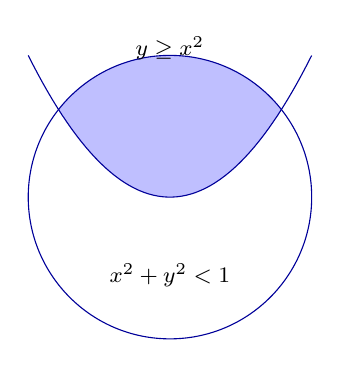
\begin{tikzpicture}[scale=1.8]
      \begin{scope}
        \clip (0,0) circle (1);
        \clip plot[domain=-1.1:1.1,samples=60] (\x,{\x*\x}) -- (1.1,1.3) -- (-1.1,1.3) -- cycle;
        \fill[blue!25] (-1.3,-1.3) rectangle (1.3,1.3);
      \end{scope}
      \draw[blue!60!black] (0,0) circle (1);
      \draw[blue!60!black,domain=-1:1,samples=60] plot (\x,{\x*\x});
      \node at (0,-0.55) {\footnotesize $x^2+y^2<1$};
      \node at (0,1.05) {\footnotesize $y \geq x^2$};
    \end{tikzpicture}
    \end{center}
  \item Since $x^3-x = x(x+1)(x-1) \geq 0$ exactly for $x \in [-1,0]\cup[1,\infty)$, the curve
    $y = \pm\sqrt{x^3-x}$ is only real on these two intervals; $B$ is the union of the graphs of
    $f(x) := \sqrt{x^3-x}$ and $-f(x)$, giving a closed loop over $[-1,0]$ and an unbounded branch
    over $[1,\infty)$ growing like $x^{3/2}$. Note that the two branches meet exactly where
    $f = 0$, i.e.\ at the three roots $x = -1, 0, 1$, which is why the loop closes up and the
    right branch starts with a vertical tangent.
    \begin{center}
    % Generator: Claude Opus 5 (High) --- FIG-W01-01.
    % Sign check: x^3-x = x(x-1)(x+1) >= 0 on [-1,0] and on [1,infty).
    % Max of x^3-x on [-1,0] is at x = -1/sqrt3 = -0.577, value 0.385, so |y| <= 0.62 there.
    \begin{tikzpicture}[>=Latex, scale=1.15]
      \draw[->] (-1.6,0) -- (2.15,0) node[right, font=\small] {$x$};
      \draw[->] (0,-2.25) -- (0,2.45) node[above, font=\small] {$y$};
      \draw (-1,0.06) -- (-1,-0.06) node[below left, font=\footnotesize] {$-1$};
      \draw (1,0.06) -- (1,-0.06) node[below right, font=\footnotesize] {$1$};

      \draw[blue!60!black, thick, domain=-1:0, samples=120]
        plot (\x, {sqrt(abs(\x*\x*\x-\x))});
      \draw[blue!60!black, thick, domain=-1:0, samples=120]
        plot (\x, {-sqrt(abs(\x*\x*\x-\x))});
      \draw[blue!60!black, thick, domain=1:1.8, samples=120]
        plot (\x, {sqrt(abs(\x*\x*\x-\x))});
      \draw[blue!60!black, thick, domain=1:1.8, samples=120]
        plot (\x, {-sqrt(abs(\x*\x*\x-\x))});

      \fill (-1,0) circle (1.3pt);
      \fill (0,0) circle (1.3pt);
      \fill (1,0) circle (1.3pt);
      % Labels are kept clear of the curve: the loop never exceeds |y| = 0.62, the strip
      % 0 < x < 1 is empty, and the right branch reaches y = 1.75 only at x = 1.63.
      \node[font=\footnotesize, blue!60!black, align=center] at (-0.72,1.3)
        {closed loop\\ over $[-1,0]$};
      % Both kept off the curve: at height y the right branch sits at x with x^3-x = y^2,
      % so y = 1.30 puts it at x = 1.44 and the label starts only at x = 1.95.
      \node[font=\footnotesize, blue!60!black, align=left, anchor=west] at (1.95,1.30)
        {unbounded branch,\\ $\sim x^{3/2}$};
      \node[font=\footnotesize, gray, align=left, anchor=west] at (-1.62,-1.55)
        {no real points\\ for $0<x<1$};
    \end{tikzpicture}
    \end{center}
    % Generator: Claude Sonnet 5 (Medium) --- the solution continues below; only the figure
    % above is an addition.
  \item Since $0 < x < y$, points of $C$ lie in the first octant with $y > x$; the condition
    $\pi/6 < \arctan(y/x) < \pi/3$ says the angle to the positive $x$-axis is between $30^\circ$
    and $60^\circ$. So $C$ is the open angular sector between the lines $y=x$ and $y=\sqrt{3}\,x$:
    \begin{center}
    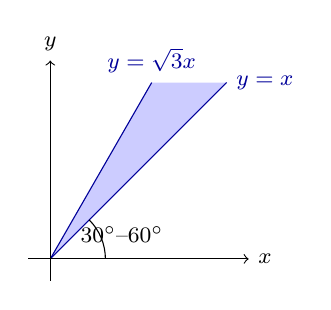
\begin{tikzpicture}[scale=1.4]
      \fill[blue!20] (0,0) -- (1.6,1.6) -- (0.92,1.6) -- cycle;
      \draw[blue!60!black] (0,0) -- (1.6,1.6) node[right] {\footnotesize $y=x$};
      \draw[blue!60!black] (0,0) -- (0.92,1.6) node[above] {\footnotesize $y=\sqrt{3}x$};
      \draw[->] (-0.2,0) -- (1.8,0) node[right] {\footnotesize $x$};
      \draw[->] (0,-0.2) -- (0,1.8) node[above] {\footnotesize $y$};
      \draw (0.5,0) arc (0:45:0.5);
      \node at (0.65,0.22) {\footnotesize $30^\circ$--$60^\circ$};
    \end{tikzpicture}
    \end{center}
  \item Slicing at height $z=t \in (0,1)$: the equation $\sqrt{x^2+y^2} = 1-t$ describes a circle
    of radius $1-t$ centered on the $z$-axis. As $t$ ranges over $(0,1)$, the radius shrinks
    linearly from $1$ to $0$, so $D$ is the lateral surface of a right circular cone of height $1$
    over the unit circle, apex at $(0,0,1)$, base circle excluded (the inequalities are strict).
  \item Slicing at height $z=t$: the equation $\sqrt{1+x^2+y^2}=t$ has solutions only for
    $t \geq 1$, and the slice is then a circle of radius $\sqrt{t^2-1}$. Note that the radius is
    $\sqrt{t^2-1}$ and not $t$; this is the single most common slip on this part, and it turns the
    answer into a cone. $E$ is instead a bowl-shaped surface of revolution with vertex at
    $(0,0,1)$, obtained by rotating the curve $y = \sqrt{1+x^2}$ about the $z$-axis. It approaches
    slope $1$ for large $x,y$ without ever attaining it, which is exactly how it differs from the
    cone $z = \sqrt{x^2+y^2}$ that it is so often mistaken for.
  \item The level sets $\{\max\{|x|,|y|\}=t\}$ are the boundaries of the squares $[-t,t]^2$.
    Stacking these square outlines at height $z=t$ as $t$ grows from $0$ upward sweeps out four
    flat triangular faces meeting at the apex $(0,0,0)$. So $F$ is an upward-opening
    \emph{square cone}: the exact analogue of the circular cone of part \textbf{(d)}, with the
    round level circles of $\sqrt{x^2+y^2}$ replaced by the square level curves of
    $\max\{|x|,|y|\}$.
\end{enumerate}

Parts \textbf{(d)}, \textbf{(e)} and \textbf{(f)} are the same construction carried out three
times, stacking level sets, and are best compared side by side. In each panel the dotted curve is
one intermediate level set:

\begin{center}
% Generator: Claude Opus 5 (High) --- FIG-W01-02.
% Oblique projection: a horizontal circle of radius R is drawn as an ellipse (R and 0.34*R).
% (4) apex (0,0,1) at the top, radius 1-z, so radius 1 at z=0: a downward-opening cone.
% (5) z = sqrt(1+x^2+y^2): vertex (0,0,1), radius sqrt(z^2-1); at z=2 the radius is sqrt3=1.73.
% (6) z = max(|x|,|y|): apex at the origin, level sets are SQUARES of half-side z.
\begin{tikzpicture}[>=Latex, scale=0.95]

  % ---------- Panel (4): circular cone, apex up ----------
  \begin{scope}[shift={(0,0)}]
    \draw[->] (0,-0.35) -- (0,2.5) node[above, font=\footnotesize] {$z$};
    \draw[blue!70!black, thick] (0,2.0) -- (-1.3,0);
    \draw[blue!70!black, thick] (0,2.0) -- (1.3,0);
    \draw[blue!70!black, thick, dashed] (0,0) ellipse (1.3 and 0.44);
    \draw[blue!70!black, dotted] (0,1.0) ellipse (0.65 and 0.22);
    \fill (0,2.0) circle (1.5pt) node[above right, font=\footnotesize] {$(0,0,1)$};
    \node[font=\footnotesize, align=center] at (0,-1.0)
      {\textbf{(d)} $\sqrt{x^2+y^2}=1-z$\\ radius shrinks $1 \to 0$};
  \end{scope}

  % ---------- Panel (5): bowl, opening upward ----------
  \begin{scope}[shift={(4.4,0)}]
    \draw[->] (0,-0.35) -- (0,2.5) node[above, font=\footnotesize] {$z$};
    % asymptotic cone z = |x| (slope 1), drawn from the origin
    \draw[gray!65, dashed] (-1.9,1.9) -- (0,0) -- (1.9,1.9);
    \draw[blue!70!black, thick, domain=-1.75:1.75, samples=80]
      plot (\x, {sqrt(1+\x*\x)});
    \draw[blue!70!black, thick] (0,2.02) ellipse (1.75 and 0.30);
    \draw[blue!70!black, dotted] (0,1.41) ellipse (1.0 and 0.20);
    \fill (0,1.0) circle (1.5pt) node[below right, font=\footnotesize] {$(0,0,1)$};
    \node[gray!70!black, font=\footnotesize, anchor=west] at (1.2,0.45) {$z=|x|$};
    \node[font=\footnotesize, align=center] at (0,-1.0)
      {\textbf{(e)} $z=\sqrt{1+x^2+y^2}$\\ radius $\sqrt{z^2-1}$, \emph{not} $z$};
  \end{scope}

  % ---------- Panel (6): square cone, apex at the origin ----------
  \begin{scope}[shift={(8.8,0)}]
    \draw[->] (0,-0.35) -- (0,2.5) node[above, font=\footnotesize] {$z$};
    % the four corners of the square [-t,t]^2 at height t=2, in the same oblique projection
    \coordinate (c1) at (1.3,2.44);
    \coordinate (c2) at (1.3,1.56);
    \coordinate (c3) at (-1.3,1.56);
    \coordinate (c4) at (-1.3,2.44);
    \draw[blue!70!black, thick] (c1) -- (c2) -- (c3) -- (c4) -- cycle;
    \foreach \c in {(c1),(c2),(c3),(c4)}{\draw[blue!70!black, thick] (0,0) -- \c;}
    \draw[blue!70!black, dotted] (0.65,1.22) -- (0.65,0.78) -- (-0.65,0.78) -- (-0.65,1.22) -- cycle;
    \fill (0,0) circle (1.5pt) node[below right, font=\footnotesize] {$(0,0,0)$};
    \node[font=\footnotesize, align=center] at (0,-1.0)
      {\textbf{(f)} $z=\max\{|x|,|y|\}$\\ squares instead of circles};
  \end{scope}
\end{tikzpicture}
\end{center}
\end{exercisesolution}

\begin{exercisesolution}[Solution of \cref{ex:drawings_to_equations}]
\label{sol:drawings_to_equations}
% Generator: Claude Sonnet 5 (Medium)
\begin{enumerate}[label=\textbf{(\alph*)}]
  \item A point moving back and forth along the segment from $(0,0)$ to $(-1,1)$ can be
    parametrized as $t \mapsto (-f(t), f(t))$ for $t \geq 0$, where $f : [0,\infty) \to [0,1]$
    oscillates endlessly; $f(t) := \tfrac{1}{2}(1+\sin t)$ is one valid choice.
  \item Remove two small disjoint squares from a large square, e.g.
    $\{10 > \max\{|x|,|y|\} > 1\} \setminus \{\max\{|x-5|,|y-6|\} \leq 1\}$.
  \item Intersect the closed unit ball with the plane: $\{x^2+y^2+z^2 \leq 1\} \cap \{x+y+z=0\}$.
  \item Remove a $60^\circ$ wedge from a disk:
    $\{x^2+y^2 \leq 1\} \setminus \{|\arctan(y/x)| \leq \pi/6,\ x>0\}$.
  \item Combining the square level sets from \cref{ex:equations_to_drawings} part \textbf{(f)} with the conical
    slicing from part \textbf{(d)}: $\{1-z = \max\{|x|,|y|\},\ 0 \leq z \leq 1\}$ is a pyramid of
    height $1$ over the square $[-1,1]^2$, apex at $(0,0,1)$.
\end{enumerate}

The two planar answers are worth drawing, since in both cases the description \qt{remove a piece}
translates directly into a set difference:

\begin{center}
% Generator: Claude Opus 5 (High) --- FIG-W01-03.
\begin{tikzpicture}[>=Latex, scale=1.0]

  % ---------- Panel 2: square annulus with a second square removed ----------
  % Matches the formula above exactly. The outer square is max{|x|,|y|} < 10 (drawn with
  % half-side 1.5, i.e. one figure unit = 6.67 units of the formula); the FIRST hole is the
  % central max{|x|,|y|} <= 1, the SECOND is the square of half-side 1 centred at (5,6),
  % i.e. at (0.75, 0.90) in figure coordinates. Both holes therefore have half-side 0.15.
  \begin{scope}[shift={(0,0)}]
    \fill[blue!12] (-1.5,-1.5) rectangle (1.5,1.5);
    \draw[blue!60!black, thick] (-1.5,-1.5) rectangle (1.5,1.5);
    \fill[white] (-0.15,-0.15) rectangle (0.15,0.15);
    \draw[blue!60!black, thick] (-0.15,-0.15) rectangle (0.15,0.15);
    \fill[white] (0.60,0.75) rectangle (0.90,1.05);
    \draw[blue!60!black, thick] (0.60,0.75) rectangle (0.90,1.05);
    \node[font=\scriptsize, anchor=east] at (-0.26,0) {hole at $0$};
    \node[font=\scriptsize, anchor=west] at (0.99,0.90) {hole at $(5,6)$};
    \node[font=\scriptsize, align=center, anchor=north] at (0,-1.72)
      {\textbf{2.} a domain with two holes:\\
       $\{10>\max\{|x|,|y|\}>1\}$\\ minus a unit square at $(5,6)$};
  \end{scope}

  % ---------- Panel 4: Pac-Man ----------
  \begin{scope}[shift={(5.5,0)}]
    % disk minus the 60-degree wedge |arctan(y/x)| <= pi/6, x > 0
    \fill[blue!12] (0,0) -- (30:1.5) arc (30:330:1.5) -- cycle;
    \draw[blue!60!black, thick] (0,0) -- (30:1.5) arc (30:330:1.5) -- cycle;
    % the removed wedge, dashed
    \draw[red!70!black, thick, dashed] (0,0) -- (30:1.5);
    \draw[red!70!black, thick, dashed] (0,0) -- (-30:1.5);
    \draw[red!70!black, dotted] (0.55,0) arc (0:30:0.55);
    \node[red!70!black, font=\footnotesize, anchor=west] at (1.0,0.0) {$60^\circ$ wedge removed};
    \fill (0,0) circle (1.2pt);
    \node[font=\scriptsize, align=center, anchor=north] at (0,-1.72)
      {\textbf{4.} Pac-Man: the closed unit disk\\ minus the wedge
       $\{|\arctan(y/x)|\leq\pi/6,\ x>0\}$};
  \end{scope}
\end{tikzpicture}
\end{center}
\end{exercisesolution}

\begin{exercisesolution}[Solution of \cref{ex:youngs_inequality}]
\label{sol:youngs_inequality}
% Generator: Claude Sonnet 5 (Medium); display re-broken into align* by Claude Opus 5 (High).
Parts \textbf{(a)} and \textbf{(b)} are exactly the proof of \cref{prop:youngs_inequality} above.
For the bonus vector version, apply the scalar inequality coordinatewise, with $|a_i|$ in place of
$a$ and $|b_i|$ in place of $b$, and sum over $i$:
\begin{align*}
  \langle a,b\rangle
    &\ \leq\ \sum_{i=1}^n |a_i|\,|b_i|
     \ \leq\ \sum_{i=1}^n \left(\frac{|a_i|^p}{p} + \frac{|b_i|^q}{q}\right) \\[0.4ex]
    &\ =\ \frac{1}{p}\sum_{i=1}^n |a_i|^p + \frac{1}{q}\sum_{i=1}^n |b_i|^q
     \ =\ \frac{\|a\|_p^p}{p} + \frac{\|b\|_q^q}{q}.
\end{align*}
Note that the two sums separate only because the right-hand side of Young's inequality is a
\emph{sum} of powers rather than a product; this is precisely the feature that
\cref{rem:young_to_hoelder} then removes by rescaling.
\end{exercisesolution}

